
We have developed a simple simulation tool to evaluate the model
that is publicly available from (URL removed for blind-review).

\subsection{Simulation settings}

The simulation setting is shown in Figure~\ref{fig:topology-simple}.
\begin{itemize}
  \item		job: mean duration:4sec, mean 1 unit,
        frontend 1, backend 2 for data intensive job,
        frontend 2, backend 1 for interactive job,
  \item		node: capacity 100 for MDC, 1000 for DC
  \item		link: capacity 200 for MDC-DC, 1000 for DC-DC
\end{itemize}

\begin{figure}[tb]
  \begin{center}
    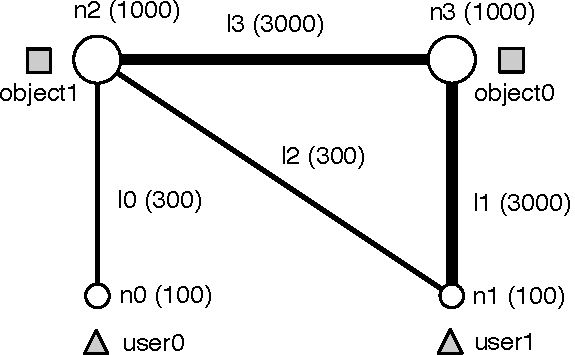
\includegraphics[width=7.5cm,clip]{topology-simple.pdf}
    \vspace{-2.0ex}
    \caption{simple simulation topology}
    \Description{Simulation topology with 2 datacenters and 2 micro datacenters.}
    \label{fig:topology-simple}
  \end{center}
\end{figure}

Simulation scenarios:
\begin{enumerate}
  \item	{\bf node only:} 4 nodes without randomization to show how the
        cost function works
  \item	{\bf link only:} 4 links without randomization to show
        different costs affects
  \item	{\bf monotonic function:} same as above but use monotonic cost
        function.
  \item	{\bf randomize:} 4 nodes and 4 links with randomization
  \item {\bf comparison:} compared with, no idle-resource pooling
  \item	{\bf surge:} same as above but with a request surge at one location
  \item	{\bf edge computing:} 2 nodes (big and small) and 1 link, the
    users are closer to the small node. 2 types jobs (interactive,
    data intensive).  show interactive jobs are on the small node,
    data intensive jobs are on the big node.
  \item {\bf premium service:} 4 nodes with 3 standard and 1 premium services.
  \item	{\bf complex?:} realistic scenario
\end{enumerate}

We use 3 types of time-series plots: one for the load of each node
(computing resource), another for the load of each link, and the last
one to show the total active jobs normalized to MDC's capacity.

\subsection{Basic Behaviors}

\begin{figure}[tb]
  \begin{center}
    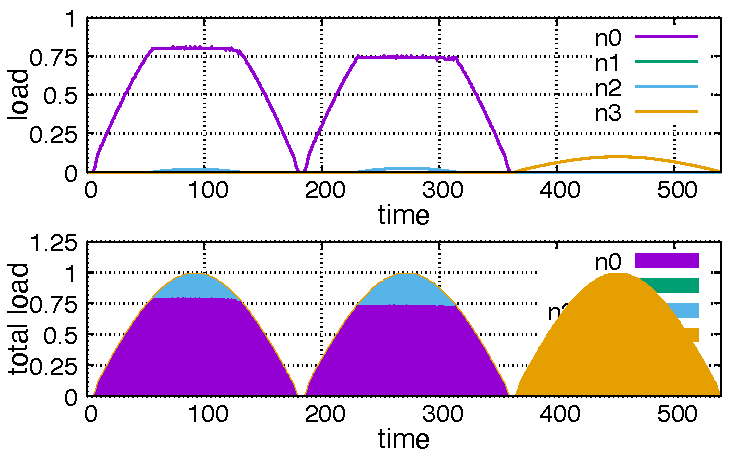
\includegraphics[width=1.0\columnwidth]{lowering.pdf}
    \vspace{-2.0ex}
    \caption{lowering load, interactive jobs vs. data intensive jobs}
    \Description{Simulation results with basic behaviors.}
    \label{fig:lowering}
  \end{center}
\end{figure}

The effects of manipulating the cost function and the job
specification is shown in Figure~\ref{fig:lowering}.
A series of jobs are generated between a user at MDC0 and an object at DC3.
The first and second waves contain only interactive jobs, and most of
the jobs are assigned to the node closest to the user (MDC0) but some
overflowing jobs are assigned to DC2.
In the second wave, the cost function of MDC0 is manipulated to reduce
the load by multiplying the cost function by 1.5.
The third wave contains only data intensive jobs, and all jobs are
assigned to the node that has the object (DC3).

\subsection{Mixed Behaviors}

A more complex scenario is shown in Figure~\ref{fig:mixed}.
user0: cycle: 180  peak:1.2 interactive:data-intensive=1:2.
user1: cycle: 135  peak:1.0  interactive:data-intensive=1:3.
after time 540 (5th wave for user1), user1 load x 2.0, 
after time 675 (6th wave for user1), user1 load x 10.
before, time 540, interactive jobs are assigned closer to the user,
and data intensive jobs are assigned closer to the data.
For the 6th wave, n1 saturates, then assigned to n2 but the link to n2
saturates, and the rest assigned to n3.

\begin{figure}[tb]
  \begin{center}
    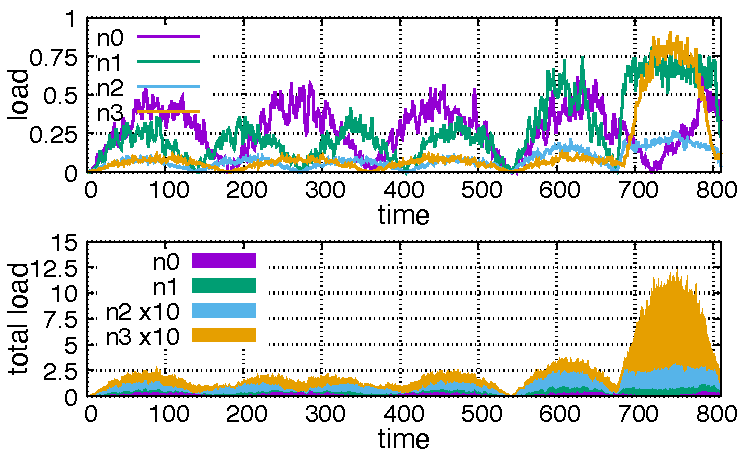
\includegraphics[width=1.0\columnwidth]{simu2.pdf}
    \vspace{-2.0ex}
    \caption{mixed scenario}
    \Description{Simulation results with mixed scenario.}
    \label{fig:mixed}
  \end{center}
\end{figure}

% \begin{figure}[tb]
%   \begin{center}
%     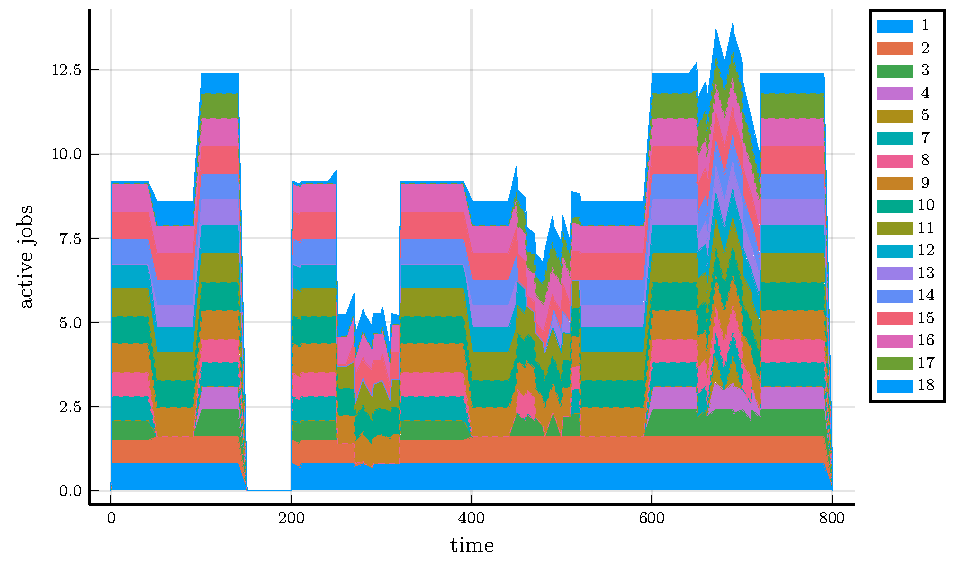
\includegraphics[width=1.0\columnwidth]{complex-convex-monotonic.pdf}
%     \vspace{-2.0ex}
%     \caption{Complex scenario with convex nodes and monotonic links}
%     \label{fig:complex}
%   \end{center}
% \end{figure}

% \begin{figure}[tb]
%   \begin{center}
%     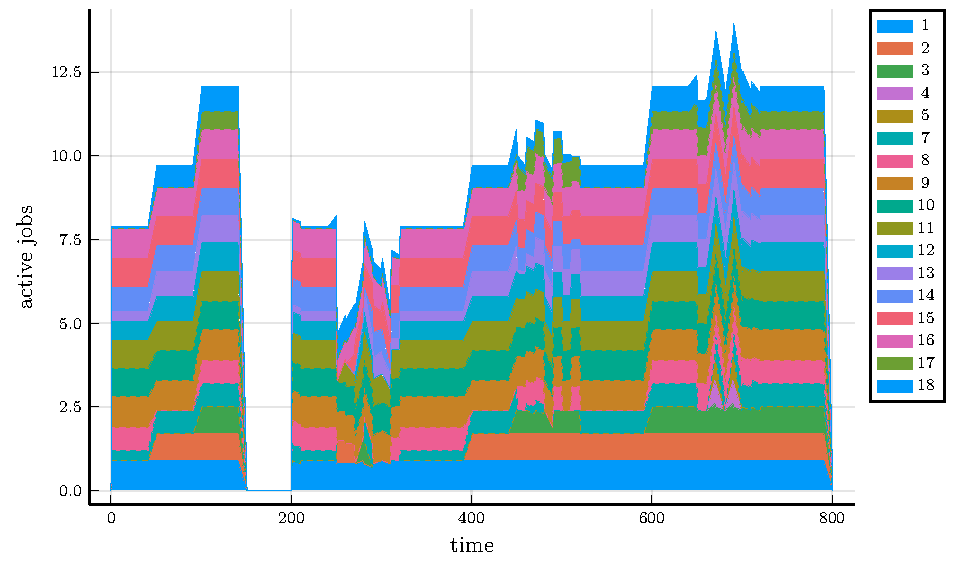
\includegraphics[width=1.0\columnwidth]{complex-full-convex.pdf}
%     \vspace{-2.0ex}
%     \caption{Complex scenario with convex nodes and monotonic links}
%     \label{fig:complex-convex}
%   \end{center}
% \end{figure}

% \begin{figure}[tb]
%   \begin{center}
%     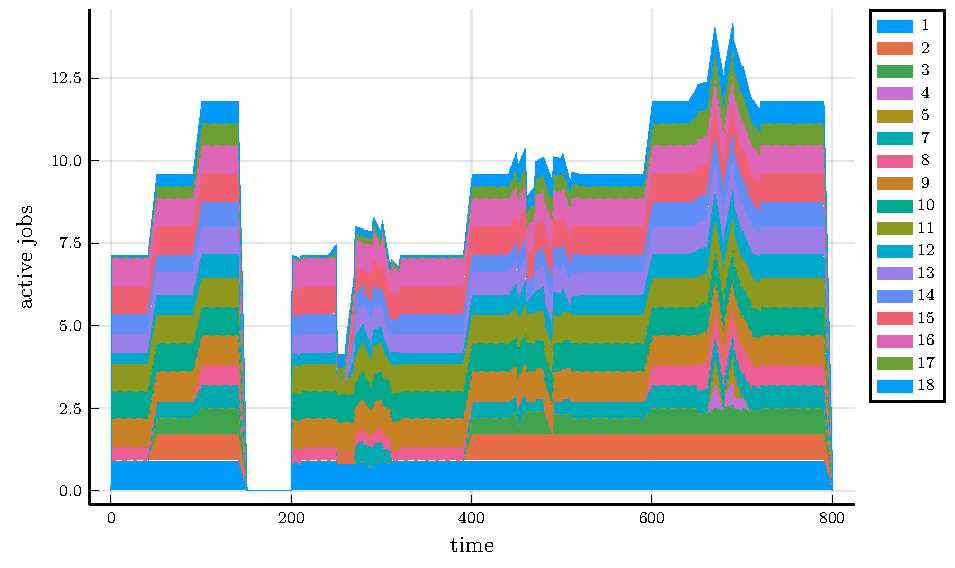
\includegraphics[width=1.0\columnwidth]{complex-full-monotonic.pdf}
%     \vspace{-2.0ex}
%     \caption{Complex scenario with convex nodes and monotonic links}
%     \label{fig:complex-monotonic}
%   \end{center}
% \end{figure}

\begin{figure}[tb]
  \centering
  \begin{subfigure}{\columnwidth}
      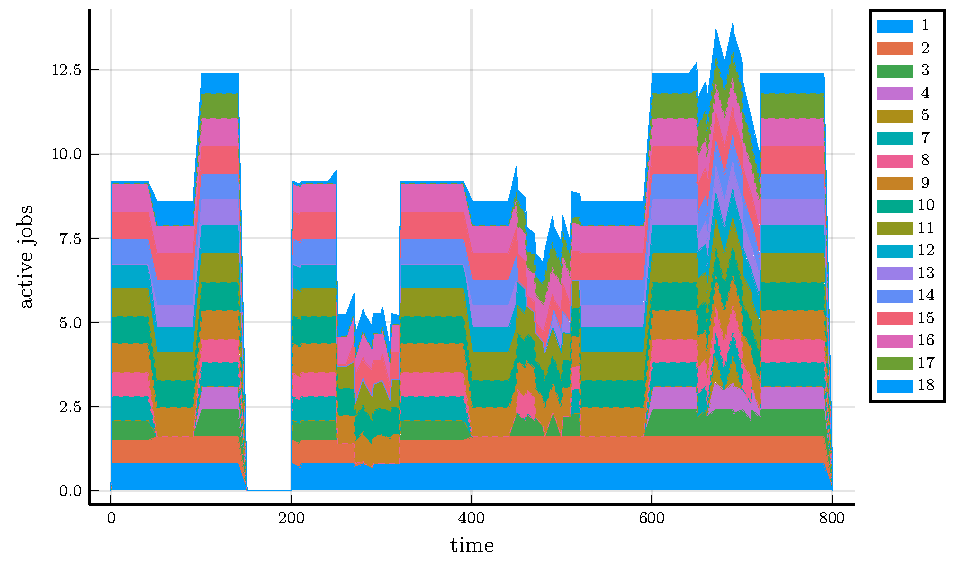
\includegraphics[width=\textwidth]{complex-convex-monotonic.pdf}
      \caption{Convex nodes and monotonic links}
      \label{fig:first}
  \end{subfigure}

  \begin{subfigure}{\columnwidth}
      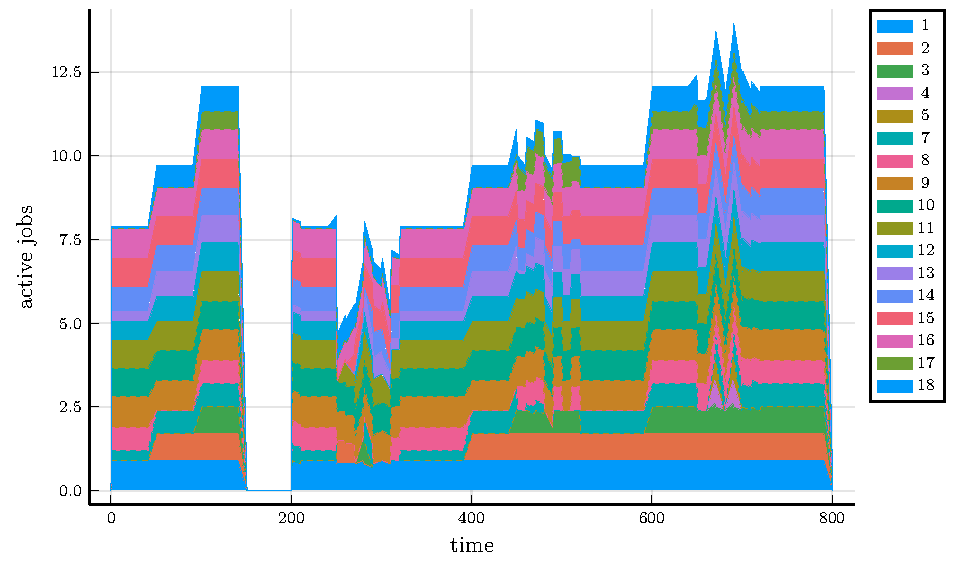
\includegraphics[width=\textwidth]{complex-full-convex.pdf}
      \caption{Convex nodes and links}
      \label{fig:second}
  \end{subfigure}

  \begin{subfigure}{\columnwidth}
      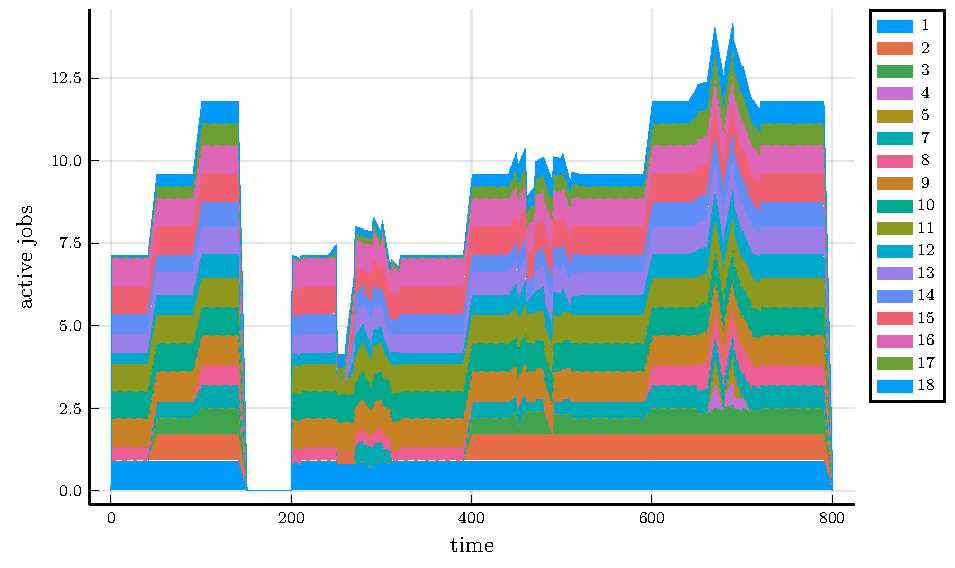
\includegraphics[width=\textwidth]{complex-full-monotonic.pdf}
      \caption{Monotonic nodes and links}
      \label{fig:third}
  \end{subfigure}

  \caption{Comparison of convex and monotonic resources in a complex scenario}

  \label{fig:figures}
  \end{figure}